\chapter{Breezy Project: a DOTA 2 competition}
\label{chap:dota}

During the first month of my internship I teamed up with my supervisor \addlink{https://www.linkedin.com/in/dennis-g-wilson/}{Assoc. Prof. Dennis Wilson} and my fellow Research Intern \addlink{https://www.linkedin.com/in/lucashervier/}{Lucas Hervier} to participate in an Evolutionary Reinforcement Learning competition held as part of the international Genetic and Evolutionary Computation Conference, known as GECCO 2020, on the DOTA 2 video game. \\
The agents we submitted are available on \addlink{https://github.com/d9w/DotaBot}{GitHub}, and the source code has been \addlink{https://github.com/d9w/Project-Breezy-DOTA-Evolutionnary}{made open-source}.

\section{Context}
\subsection{Video games and Machine learning}
In 2018 the video game industry generated sales of more than US\$130 billion, reaching around 2 billion players around the world. Because video games can provide complex tasks necessitating short- and long-term planning in a controlled environment with no risks to humans \cite{Games_AI}, they also provide an excellent test-bed for Artificial Intelligence (AI) systems. Multiple learning agents have been tested on the Arcade Learning Environment based on Atari 2600 games \cite{Atari}, including Reinforcement Learning (RL) techniques like Deep Q Networks \cite{DQN} and Agent57 \cite{agent57}. Other games such as StarCraft, DOTA2, Mario, or Doom, have also been extensively used as machine learning benchmarks.

Since the reward in games is often sparse, making the learning signal weak, gradient-based methods might struggle for the optimization of neural network parameters. Evolutionary Strategies (ES), which estimate the gradient of the objective function without needing an explicit gradient definition, have been used to optimize Deep Convolutional Neural Networks \cite{CMAES_DL}, and the evolution of synaptic weights have been demonstrated to be competitive with deep RL methods\cite{deep_neuroevo}.\\

\subsection{OpenAI Five}
From 2016 to 2019, \addlink{https://openai.com/about/}{OpenAI} published work on the \addlink{https://openai.com/projects/five/}{OpenAI Five project}, an AI trained to play Dota 2 first in 1v1, and then extended to 5v5. OpenAI Five achieved a \addlink{https://arena.openai.com/#/results}{99.4\% win rate} against human players of any rank and \addlink{https://openai.com/blog/openai-five-defeats-dota-2-world-champions/}{defeated the world champions} twice in a live tournament, while also showing cooperation capabilities with humans. 

However, most of the technical details of the AIs trained for this project still remain unknown and unpublished, from the model architecture to the interface used to communicate with the game developed in partnership with Valve. Hence, further work and results reproduction are harder to implement, adding to the computational constraint (OpenAI Five required 764 petaflop/s-day operations for \textbf{over 10,000 years of games} against itself, totalling around $6.6.10^{22}$ operations). This makes the use of Dota 2 as a RL benchmark and its use in the development of open-source RL algorithms still an open problem. 

\subsection{Project Breezy}

In this context, \addlink{https://web.cs.dal.ca/~dota2/?page_id=353}{Project Breezy} is a competition created by Robert Smith and Malcolm Heywood from Dalhousie University to develop a DOTA 2-playing bot evolved with evolutionary algorithms, in a 1-versus-1 symmetrical match-up. 

For this purpose, they implemented and published a server interfacing with the Dota 2 game. As this work was not officially supported by Valve there may still be a performance difference compared to the system used to train openAI Five, but it provides an open-source tool for benchmarks.

We entered this competition as an opportunity to try and test neuroevolution algorithms on a complex real-time game, and as a step towards the development of a comprehensive benchmark of Evolutionary Reinforcement Learning algorithms as described in Chapter \ref{chap:berl}.

\section{DOTA 2 as a RL environment}
\subsection{The game}

Produced by Valve and available on its platform \addlink{https://store.steampowered.com/app/570/Dota_2/}{Steam}, \addlink{https://en.wikipedia.org/wiki/Dota_2}{Dota 2} is the sequel of Defense of the Ancients (DotA), a community-created game mod for Warcraft III that popularised the Multiplayer Online Battle in Arena (\addlink{https://en.wikipedia.org/wiki/Multiplayer_online_battle_arena}{MOBA}) video game genre. In Dota 2, 2 teams (called "Radiant" and "Dire") of 5 players compete to destroy the main structure of the enemy's base (the "Ancient") in a real-time strategy game, each player controlling one of the 119 possible characters (the "heroes").

\begin{figure}[H]
 \centering
 \captionsetup{justification=centering, margin=0.5cm}
 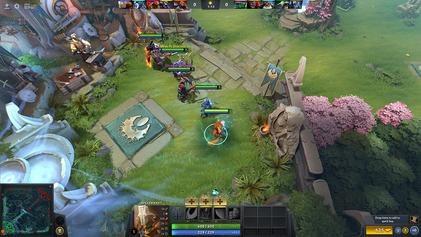
\includegraphics[width=8cm]{images/Dota_2_Gameplay_Aug_2017.jpg}
\caption{A game of Dota 2 in progress, showing the Radiant team inside their base at the beginning of a match}
 \small\textsuperscript{\url{https://en.wikipedia.org/wiki/Dota_2}}
 \label{fig:dota-2-game}
\end{figure}

The game takes place on a square map (cf fig. \ref{fig:dota-2-map}) which contains both team-controlled buildings (e.g. towers, barracks) that the other team can attack, and neutral objectives (e.g. Roshan). Team bases are situated in the bottom-left and top-right corners respectively, with 3 lanes joining them called the top (through the top-left corner), the middle (diagonally), and the bottom (through bottom-right corner) lane, each guarded by towers and around which most early gameplay happens. Creeps are basic AI-controlled units that periodically spawn for each team at the barracks and walk down the lane to help destroy enemy buildings. Dealing the last hit ("last hitting") an enemy creep is rewarded with money, which allows to buy items influencing the player's hero strengths. Last hitting a creep of the same team allows to deny them from the enemy. 

\begin{figure}[H]
 \centering
 \captionsetup{justification=centering, margin=0.5cm}
 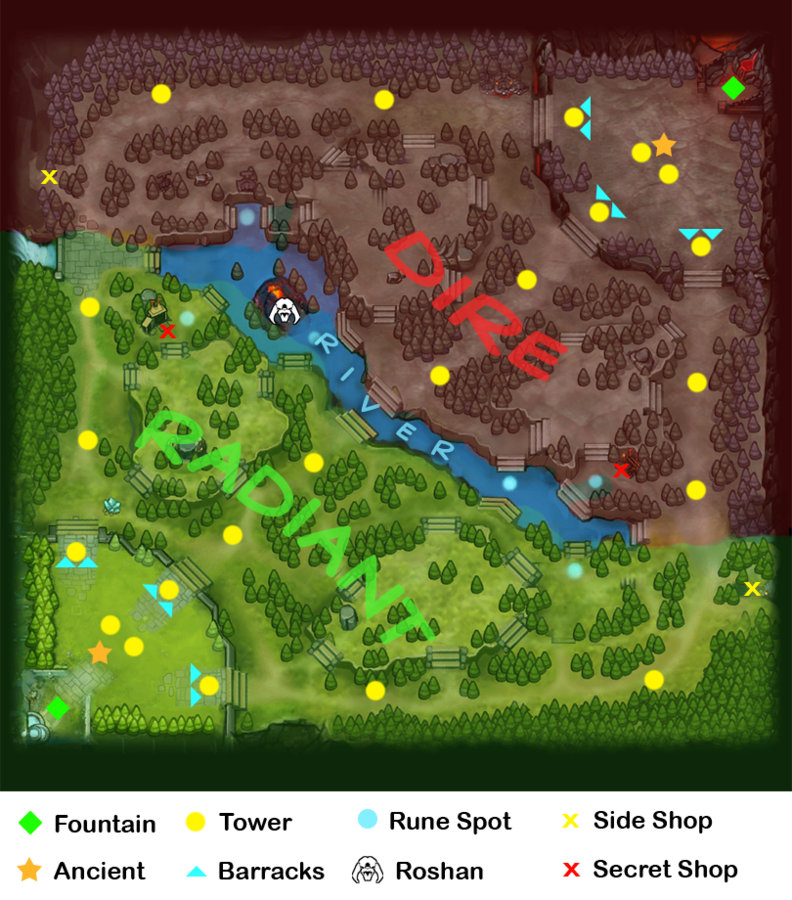
\includegraphics[width=8cm]{images/dota-map.png}
\caption{Labelled Dota 2 map as of version 7.20}
 \small\textsuperscript{\url{https://dota2.gamepedia.com/Map}}
 \label{fig:dota-2-map}
\end{figure}

The 1v1 game mode opposes only 1 player in each team, and can be won by either killing the enemy twice, or destroying the first enemy tower on the middle lane. \\
The game mode used for this competition additionally fixes the heroes to be \addlink{https://dota2.gamepedia.com/Shadow_Fiend}{Shadow Fiend} for both players, for balancing purposes.

\subsection{Project Breezy Software}
\addlink{https://web.cs.dal.ca/~dota2/?page_id=353}{Project Breezy} provides software to enable communication with the Dota 2 game by opening a server communicating with the game instance. The agent, through a Python server, interacts with the Breezy server, getting the game state and sending action orders. The game state contains 310 features such as health points, hero position, creeps positions, or spell cooldowns. 29 actions are available, including movementS, spell casting, or attacking.

We noticed the server actually returned the state before effectuating an action, adding a delay in the information processing. Even though evolved models might still work thanks to internal memory, recurrence, or implicit prediction, this made predicting the next state in the simulator and analyzing behaviors significantly harder. 

\subsection{Challenges}
\begin{minipage}{\linewidth}
Evolving Neural Networks to play Dota 2 is subject to multiple constraints:
\begin{itemize}
    \item \textbf{Processing time}: Since DOTA 2 is a real-time game, the generated neural networks needs to be fast to evaluate at each step.
    \item \textbf{Evaluation time}: Even sped up, evaluating a policy requires running a full game in a simulator, hence the number of evaluations is a strong limiting factor.
    \item \textbf{Network size}: Due to the large size of the game state provided by the Breezy server and the hight number of possible actions, generated neural networks might require large architectures, hence increasing computation time and problem dimensionality.
    \item\textbf{Network complexity}: Since Dota 2 requires both short- and long-term planning, more complex architectures might be required 
    \item \textbf{Fitness sparsity}: Since the fitness used rewards dealing damage and last hitting, many behaviors that do not get close enough to the enemy have the same fitness, hence information about the quality of an individual is rare and requires already advanced policies
\end{itemize}
\end{minipage}

\section{Our approach}

\subsection{Problem Modeling}
\label{sec:representation choice}

\subsubsection{Fitness Function}
As in order to win a 1v1 a player needs to either kill the opponent twice or to take his first mid tower, we took into account the number of times we killed the opponent champion and the opponent tower health in the individual evaluation. Moreover, to succeed in one of those two tasks one would also need good laning skills, so we also added the amount of gold collected (\textit{net worth}), the number of last hits, and the number of denies. We also punished being killed and behaviors causing an early stopping as referenced in section \ref{sub:early-stop}.

\begin{minipage}{\linewidth}
The final fitness function is hence as follows:

\begin{equation*}
\label{eq:fitness}
\begin{minipage}{0.7\textwidth}
% \begin{multline*}
\begin{split}
 fitness & = netWorth + 100*lastHits + 100*denies\\
         & + 2000*ratioTowerHealth + 1000*nbKill\\
         & - 250*nbDeath - 500*earlyStop\\
 \end{split}
% \end{multline*}
\end{minipage}
\end{equation*}
\end{minipage}


\subsubsection{Behavior Space}
Our goal with a Quality-Diversity approach was to observe individuals with highly diverse behaviors to increase our chances of finding interesting ones. Therefore, we needed a characterization of the behavior space to differenciate playstyles. 
We described the behavior in a discretized 2-dimensional space featuring the \textit{total damage made to the opponent champion} and the \textit{percentage of the opponent tower health taken} as axes, since the objective was either to kill the opponent champion or to take his tower. 

\subsection{Reducing the evaluation cost}
We quickly realized that one of the main difficulty of this challenge was to deal with the evaluation cost of the fitness. Indeed, in order to evaluate an agent we need him to play a full DOTA2 game which can take up to several minutes in real time, even with a tenfold speeding. Since Evolutionnary Algorithms (EAs) require a large number of function evaluations, we had to find a way to cope with this issue. 

\subsubsection{Early stopping}
\label{sub:early-stop}
A simple but efficient way of reducing the evaluation time was to use an Early Stopping mechanism. We decided to stop the evaluation of an agent if he did not kill a creep after 5min of DOTA time. This functionality reduced the time loss due to static individual, and the evaluation length of "coward individuals" avoiding fights.

\subsubsection{Neural-base simulator}
Since an evaluation is time consuming, I developped a \addlink{https://github.com/TemplierPaul/Dota_Simulator}{\textbf{Dota Simulator}} to predict game state evolutions from previous state and chosen action, using a neural network trained on more than 100 games played with a random policy.

The  main part of the simulator was implemented in object-orient Python to process game data, remove constant features to reduce the size of the network, create and train the neural network, and act as a simulator with a Gym-like API. A Julia wrapper was then added, to allow plugging the simulator into the rest of the project.\\
Jupyter notebooks were also used to explore data and train the networks on the \addlink{https://research.google.com/colaboratory/local-runtimes.html?hl=en}{Google Colaboratory} platform.  

3 networks of growing depths based on the UNet \cite{unet} architecture, and simple feed-forward neural networks were tried, with no particular performance difference observed. Finally, a feed-forward network with few layers of many neurons was chosen.  

\begin{figure}[H]
 \centering
 \captionsetup{justification=centering, margin=0.5cm}
 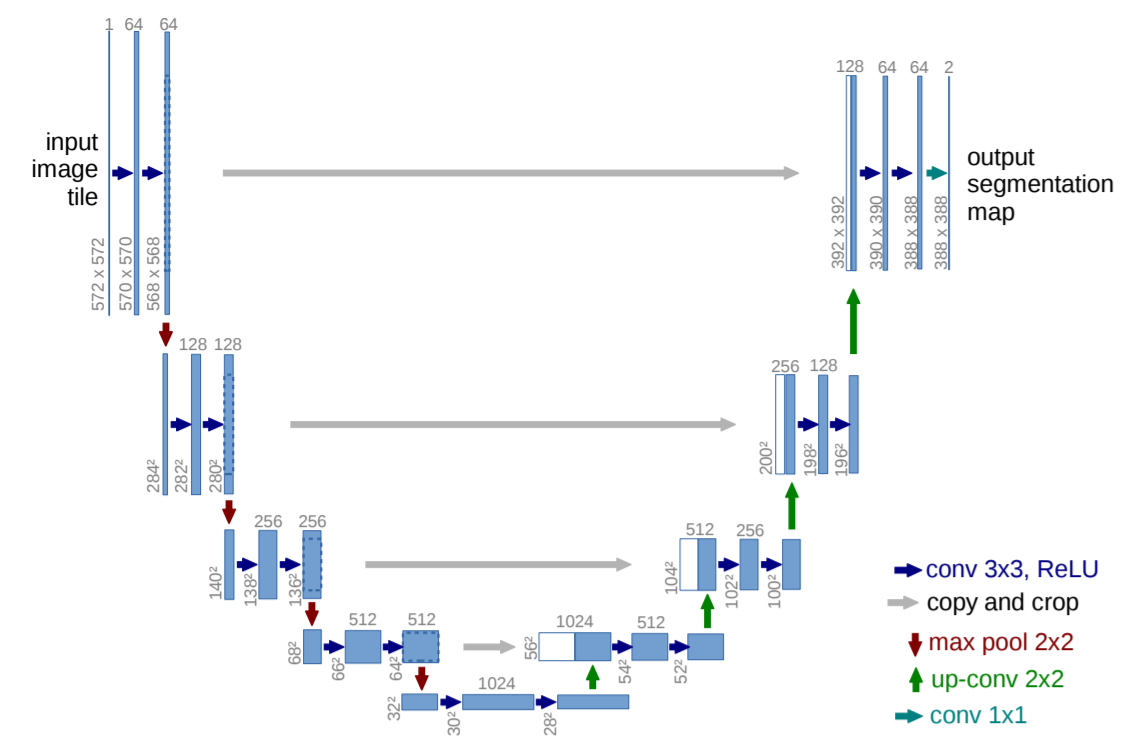
\includegraphics[width=8cm]{images/unet.PNG}
\caption{Example U-net architecture in \cite{unet}, each blue box corresponding to a multi-channel feature map.}
 \label{fig:dota-2-map}
\end{figure}

The simulator was used in the offsprings generation phase to encourage diversity:
\begin{itemize}
    \item offsprings are generated for 10 times the size of population 
    \item 100 game steps are simulated for each offspring, and the actions taken at each step are stored
    \item the actions taken by each individual are used to select the \textit{population size} most unique offsprings based on behavior
    \item those individuals are added to the new population and evaluated in the real game to compute the real fitness
\end{itemize}

By doing so we are seeing much more mutation and/or crossover. Moreover, taking the individuals the more distant from each other increases our chances to cover the behavior space.

\subsection{Algorithms}
We chose to train both CGP Individuals  \cite{CGP} and NEAT Individuals \cite{NEAT_1}, as defined in the respective papers, in a MAP-Elites algorithm. They were implemented with \href{https://github.com/d9w/CartesianGeneticProgramming.jl}{\textbf{CartesianGeneticProgramming.jl}} for the CGP agent, and a custom NEAT agent developed at \href{https://github.com/d9w/NEAT.jl}{\textbf{NEAT.jl}} for this challenge.

As we believed the best way to find interesting individuals, either with NEAT or with CGP, was to explore the behavorial space, we based the exploration on the \textbf{Illuminating search spaces by mapping elites} \cite{MapElites} work, implementing a MAP-Elites method to find policies of varying styles, focusing more on killing the enemy, on destroying the tower, or balancing both. 
As the evaluation of a policy relies on a full game which can be heavily influenced by small perturbations, including time delays due to the Breezy software communication method, the behavior space can be seen as a noisy domain. Hence, we believe using the work of \cite{noisy-map-elites} on MAP-Elites in noisy domains using deep grids to consider this property and  make the evaluation more reliable could improve future work, since it was published too late for us to implement it. 

\section{Results}

Results were announced at GECCO 2020 on July 12\textsuperscript{th} by the organizers. \\
9 teams had registered to the competition, but only 2 -including us- provided code to be evaluated, among which we ranked first. \\

\begin{figure}[H]
\centering
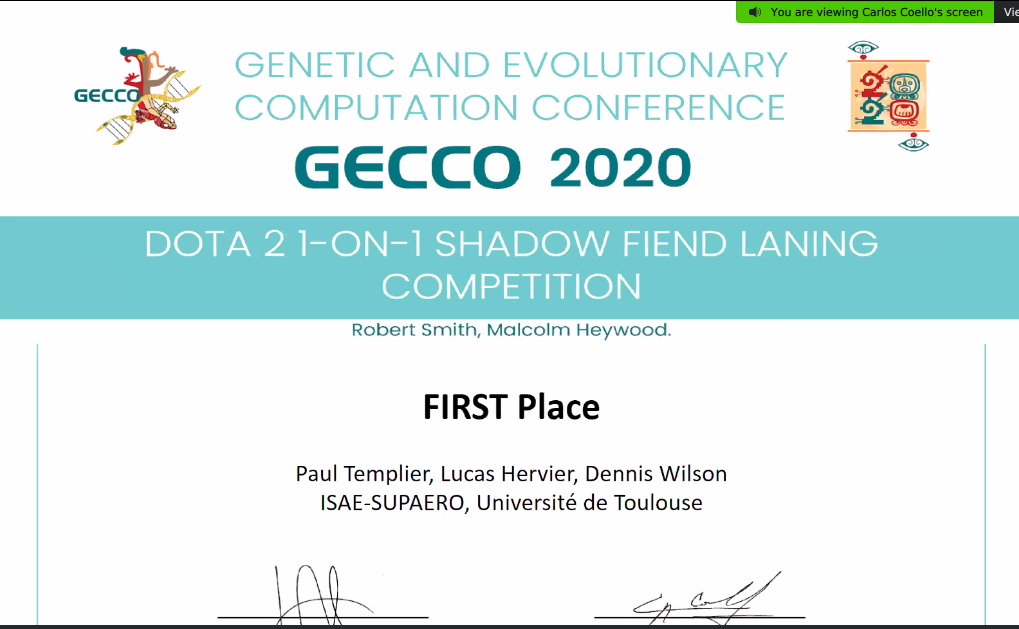
\includegraphics[width=12cm]{images/breezy-win.png}
\caption{Competition results announcement at GECCO 2020}
\end{figure}

%%% Local Variables: 
%%% mode: latex
%%% TeX-master: "isae-report-template"
%%% End: 